\section{Transformer-based Models} \label{sec:transformers}

The development of the Transformer architecture based on the \textbf{attention}
mechanism has revolutionized the field of NLP. This architecture enabled models
to process words in parallel and incorporate context from larger parts of the
input sequence, leading to substantial improvements in language modeling
performance. The improvements seen in several tasks such as machine translation,
text summarization, and text classification, made the Transformer the
state-of-the-art architecture for language modeling \cite{wolf2020transformers}.

In the following sections, we provide an overview of the Transformer
architecture and discuss its key attention mechanism (refer to
Sec.~\ref{sec:attention}). We introduce how the Transformer architecture was
adopted by the BERT model and its optimized variant RoBERTa in
Sec.~\ref{sec:bert} and Sec.~\ref{sec:roberta}, respectively. The former has
become the ubiquitous choice for baseline NLP experiments, while the latter
forms the architectural basis for the language model developed in this thesis.

\subsection{Attention} \label{sec:attention}

To give an intuition for the need for the attention mechanism, consider the
example of the following two sentences:

\begin{enumerate}
    \item \textbf{The chicken} didn’t cross the road because \textbf{it} was too
    tired. \label{ex:chicken_tired}
    \item The chicken didn’t cross \textbf{the road} because \textbf{it} was too
    wide.
    \label{ex:road_wide}
\end{enumerate}

Recall from Sec.~\ref{subsec:word_embeddings} that for static embeddings, the
representation of a word's meaning always stays the same regardless of its
context in a sentence. For instance, the word \textit{it} is always represented
by a fixed vector which could be encoding its semantic meaning as a pronoun.
However, the pronoun has a far deeper meaning in the context of the above
sentences. In sentence~\ref{ex:chicken_tired} \textit{it} refers to the chicken,
while in sentence~\ref{ex:road_wide} \textit{it} refers to the road. Thus, in
order to compute the meaning of the sentences, we will need to associate each
word with certain words, creating \textit{contextual embeddings}. Additionally,
we have to account for large \textit{context windows}, i.e. the distance between
associated words, especially considering documents with numerous paragraphs and
sentences.

The attention technique, first proposed in \cite{bahdanau2015neural}, lies at
the core of the Transformer and provides the capabilities needed to efficiently
model the rich linguistic relationships of sequences as discussed above. It can
be thought of as a mathematical operation that computes contextual
representations for each token in a sequence by selectively attending to and
incorporating information from prior tokens in the sequence. This is achieved by
using a scoring procedure to determine a ``relevance'' score for every pair of
tokens. Attention takes an input representation $\bm{x}_i$ for the token at
position $i$ and a context window of preceding tokens $\bm{x}_1, \ldots ,
\bm{x}_{i-1}$, producing an output $\bm{a}_i$ known as \textit{attention}. Since
this technique examines the elements within the sequence itself, as opposed to
attending to an external source\footnotemark{}, it is also referred to as
\textbf{self-attention} within the framework of Transformers.

\begin{figure}[htb]
    \centering
    \resizebox*{.8\textwidth}{!}{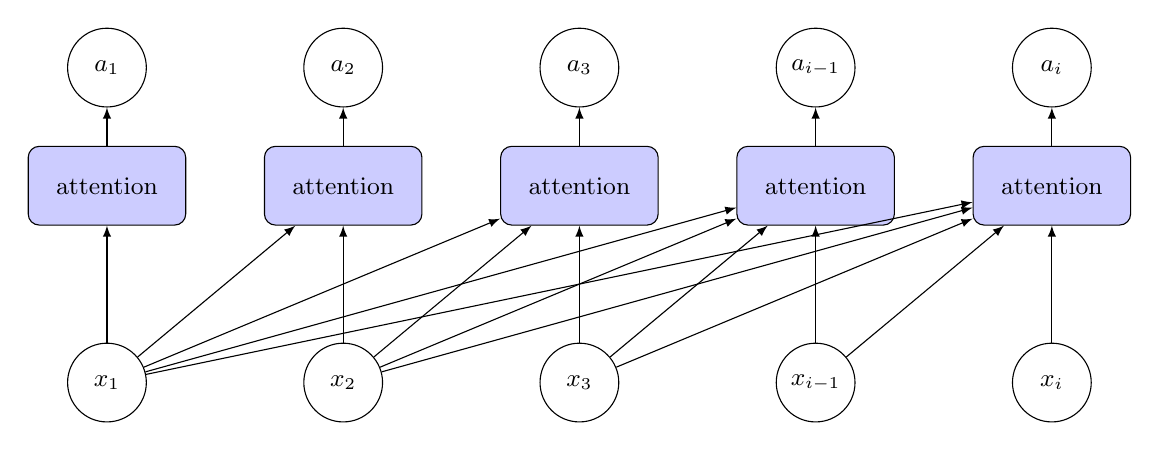
\begin{tikzpicture}[
    attention/.style={draw, fill=blue!20, rounded corners, font=\small, text centered, minimum width=2cm, minimum height=1cm},
    input/.style={draw, circle, minimum size=1cm, text centered, font=\small},
    output/.style={draw, circle, minimum size=1cm, text centered, font=\small},
    arrow/.style={->, >=latex}
]

% Inputs (x1 to x5)
\node[input] (x1) at (1, -1) {$\bm{x}_1$};
\node[input] (x2) at (4, -1) {$\bm{x}_2$};
\node[input] (x3) at (7, -1) {$\bm{x}_3$};
\node[input] (x4) at (10, -1) {$\bm{x}_{i-1}$};
\node[input] (x5) at (13, -1) {$\bm{x}_i$};

% Attention Blocks
\node[attention] (att1) at (1, 1.5) {attention};
\node[attention] (att2) at (4, 1.5) {attention};
\node[attention] (att3) at (7, 1.5) {attention};
\node[attention] (att4) at (10, 1.5) {attention};
\node[attention] (att5) at (13, 1.5) {attention};

% Outputs (a1 to a5)
\node[output] (a1) at (1, 3) {$\bm{a}_1$};
\node[output] (a2) at (4, 3) {$\bm{a}_2$};
\node[output] (a3) at (7, 3) {$\bm{a}_3$};
\node[output] (a4) at (10, 3) {$\bm{a}_{i-1}$};
\node[output] (a5) at (13, 3) {$\bm{a}_i$};

% Arrows from inputs to attention blocks
\draw[arrow] (x1) -- (att1);
\draw[arrow] (x2) -- (att2);
\draw[arrow] (x3) -- (att3);
\draw[arrow] (x4) -- (att4);
\draw[arrow] (x5) -- (att5);

% Arrows from attention blocks to outputs
\draw[arrow] (att1) -- (a1);
\draw[arrow] (att2) -- (a2);
\draw[arrow] (att3) -- (a3);
\draw[arrow] (att4) -- (a4);
\draw[arrow] (att5) -- (a5);

% Connections between inputs
\draw[arrow] (x1) -- (att2);
\draw[arrow] (x1) -- (att3);
\draw[arrow] (x1) -- (att4);
\draw[arrow] (x1) -- (att5);

\draw[arrow] (x2) -- (att3);
\draw[arrow] (x2) -- (att4);
\draw[arrow] (x2) -- (att5);

\draw[arrow] (x3) -- (att4);
\draw[arrow] (x3) -- (att5);

\draw[arrow] (x4) -- (att5);

\end{tikzpicture}
}
    \caption[Information flow in causal self-attention]{Information flow in
    causal self-attention. When processing each input $\bm{x}_{i}$, the model
    attends to all the inputs up to, and including $\bm{x}_{i}$. Figure adapted
    from \cite{jurafsky2025slp}.}
    \label{fig:attention_layer}
\end{figure}

\footnotetext{This is the case in traditional sequence-to-sequence models, where
attention would focus on another sequence, such as the target in machine
translation.}

Fig.~\ref{fig:attention_layer} depicts the outlined information flow in a
so-called \textit{causal} self-attention layer. In causal or left-to-right
language models the context window is limited to the left side of the input.
That is, for all input representations $\bm{x}_i$, the model has access to all
prior tokens $\bm{x}_j$ but no future tokens such that $j \leq i$. Notice how
this is reflected in Fig.~\ref{fig:attention_layer} at each attention function
with the information only coming from the left but not the right tokens. In
contrast, bidirectional models such as BERT (refer to Sec.~\ref{sec:bert})
generalizes attention so that it can access both past and future tokens.
Furthermore, the lack of autoregression in the attention computation allows
processing sequence tokens in parallel. Consequently, a self-attention layer
maps an input sequence $(\bm{x}_1 \ldots \bm{x}_n)$ of length $n$ to an output
sequence of the same length $(\bm{a}_1, \ldots, \bm{a}_n)$ in a single time
step, making it more efficient than recurrent mechanisms relying on
autoregression used in past language models.

\subsubsection{Scaled Dot-Product Attention}
Let us unfold the attention computation step-by-step. As mentioned, the input
token sequence consisting of a set of $n$ input embedding vectors $\bm{x}_i$ of
length $d_{model}$ is processed in parallel. To this end, the set is packed as
rows into an $n \times d_{model}$ sized matrix $\bm{X} = [\bm{x}_1^T, \ldots,
\bm{x}_n^T]$ in order to take advantage of optimized matrix multiplication
routines. The size of input embeddings is often referred to as \textbf{model
dimensionality} since it is the embedding dimension the model is able to
process, which is why the notion $d_{model}$ is used. 

The attention mechanism first projects the input embeddings $\bm{X}$ into three
different matrices $\bm{Q}$, $\bm{K}$, and $\bm{V}$. These allow the mechanism
to assign distinct roles to each input embedding throughout the attention
process:

\begin{itemize}
    \item The \textbf{query} $\bm{q}_i$ is the \textit{current element} being
    compared to the previous sequence inputs.
    \item The \textbf{key} $\bm{k}_i$ takes on the role of the \textit{preceding
    input} that is being compared to the current element in order to determine a
    relevance score.
    \item The \textbf{value} $\bm{v}_i$ is the \textit{context} that is being
    weighted and summed to form the current element's output representation.
\end{itemize}

The self-attention layer introduces weight matrices denoted by $\bm{W^Q} \in
\mathbb{R}^{d_{model} \times d_q}$, $\bm{W^K} \in \mathbb{R}^{d_{model} \times
d_k}$ and $\bm{W^V} \in \mathbb{R}^{d_{model} \times d_v}$ with $d_q = d_k$ and
$d_v$ being the size of the query, key and value vectors, respectively. These
weight matrices are model parameters to be optimized during model training and
are used to project the input embeddings $\bm{X}$ as follows:

\begin{equation}
    \label{eq:qkv_projection}
    \bm{Q} = \bm{X} \bm{W^Q}, \quad 
    \bm{K} = \bm{X} \bm{W^K}, \quad 
    \bm{V} = \bm{X} \bm{W^V}
\end{equation}

\begin{figure}[htb]
    \centering
    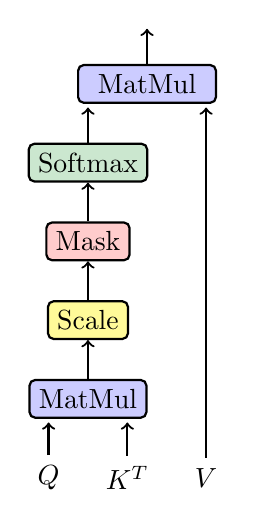
\begin{tikzpicture}[
    every node/.append style={thick,rounded corners=2pt}]
    \definecolor{softmax_color}{RGB}{203,231,207}
    \node (q) at (.5,0) {$\bm{Q}$};
    \node (k) at (1.5,0) {$\bm{K}^T$};
    \node (v) at (2.5,0) {$\bm{V}$};

    \node[draw,fill=blue!20] (matmul1) at (1,1) {MatMul};
    \node[draw,fill=yellow!40] (scale) at (1,2) {Scale};
    \node[draw,fill=red!20] (mask) at (1,3) {Mask};
    \node[draw,fill=softmax_color] (softmax) at (1,4) {Softmax};
    \node[draw, fill=blue!20, minimum width=1.75cm] (matmul2) at (1.75,5) {MatMul};

    \path[->,thick]
        (matmul1) edge (scale)
        (scale) edge (mask)
        (mask) edge (softmax)
        (q) edge (.5,.7)
        (k) edge (1.5,.7)
        (v) edge (2.5,4.7)
        (softmax) edge (1,4.7)
        (matmul2) edge[->] ++(0, .7);
\end{tikzpicture}
 
    \caption[Illustration of Scaled Dot-Product Attention]{Illustration of
    Scaled Dot-Product Attention, showing the sequential steps: MatMul between
    query $\bm{Q}$ and key $\bm{K}^T$, scaling, masking, Softmax application,
    and final MatMul with value $\bm{V}$. Figure adapted from
    \cite{vaswani2017attention}.}
    \label{fig:self_attention}
\end{figure}

Given these projections, we then compute the \textbf{Scaled Dot-Product
Attention} as shown in Fig.~\ref{fig:self_attention}. In this particular type of
attention introduced by \cite{vaswani2017attention} the dot-product is utilized
as the relevance score between query-key pairs $\bm{q}_i$ and $\bm{k}_j$.
Applying the vector dot product to the query and key matrices $\bm{Q}$ and
$\bm{K}$, results in the matrix multiplication of $\bm{Q}$ and $\bm{K}^T$. The
outcome is an $n \times n$ matrix, whose entries correspond to the relevance for
each of the possible (including non-causal) $n^2$ query-key pairs. Hence, this
matrix quantifies how much \textit{attention} should be placed on each
(projected) token embedding in the context window $n$ stored in $\bm{V}$. The
dot product grows exponentially with the model dimensionality, which leads to
numerical issues in training referred to as the \textit{exploding gradients}
\cite{pascanu2013difficulty} problem. In order to stabilize the gradients, the
score matrix is scaled by $\sqrt{d_k}$, the square root of the query and key
vector dimensionality. As briefly mentioned earlier, the $\bm{QK}^T$ matrix also
contains scores for queries $\bm{q}_i$ and keys $\bm{k}_j$ such that $j > i$. To
make the attention mechanism causal, the score matrix is masked in a way that
zeroes out the elements in the upper-triangular portion of the matrix. This is
done by adding a large negative value to the masked out elements before applying
the softmax function. The softmax function is used to normalize the scores
across the rows of the matrix, such that the weights sum up to one for each
query, i.e.

\begin{equation}
    \alpha_{ij} = \frac{\exp(\bm{q}_i \bm{k}_j^T)}{\sum_{j=1}^{n} \exp(\bm{q}_i \bm{k}_j^T)}
\end{equation}

with $\alpha_{ij}$ denoting the attention weight for the $i$-th query and $j$-th
key vector. This implies that higher scores are amplified and lower ones
diminished, giving the model more confidence in which tokens to attend to.
Lastly, the attention weights are multiplied with the value matrix $\bm{V}$ to
obtain the $n \times d_v$ sized output of the self-attention layer. More
formally, the Scaled Dot Product Attention computation is defined as:

\begin{equation}
    \label{eq:scaled_dot_product_attention}
    \text{Attention}(\bm{Q}, \bm{K}, \bm{V}) = 
    \text{softmax}\left(\frac{\bm{Q} \bm{K}^T + \bm{M}}{\sqrt{d_k}}\right) \bm{V}
\end{equation}

with $\bm{M}$ being the mask matrix where $M_{ij} = -\infty \quad \forall j > i$
and $M_{ij} = 0$ otherwise.

\subsubsection{Multi-Head Attention}
Eq.~\ref{eq:qkv_projection}-\ref{eq:scaled_dot_product_attention} describe the
computation of a single \textbf{attention head}. In practice, the Transformer
uses multiple attention heads as depicted in Fig.~\ref{fig:mh_attention}. The
intuition behind Multi-Head Attention is that different attention heads can
learn to focus on different aspects of the relationships within the input
sequence. For instance, one head might learn to focus on the subject of a
sentence, while another head might focus on the predicate or other kinds of
linguistic or even non-linguistic patterns.

\begin{figure}[htb]
    \centering
    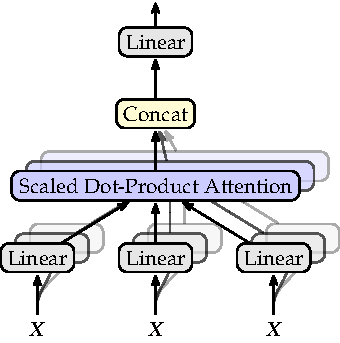
\includegraphics[width=0.4\textwidth]{mh_attention}
    \caption[Illustration of Multi-Head Attention]{Illustration of a Multi-Head
    Attention layer. Scaled Dot-Product Attention is applied $h$ times
    independently of each other and the $h$ results are concatenated to output
    the Multi-Head Attention. Figure adapted from \cite{vaswani2017attention}.}
    \label{fig:mh_attention}
\end{figure}

So in Multi-Head Attention, we learn $h$ different sets or heads of linear
projections to queries $\bm{Q}_i$, keys $\bm{K}_i$, and values $\bm{V}_i$ with
$i \in \{1, \ldots, h\}$. Thus, each head $i$ in a Multi-Head Attention layer
has its own set of projection parameters $\bm{W^Q}_i$, $\bm{W^K}_i$ and
$\bm{W^V}_i$. Subsequently, the Scaled Dot-Product Attention is applied in
parallel to each set. Finally, the $h$ sets of output are concatenated into a
single set and once again linearly projected to the model dimension $d_{model}$:

\begin{gather}
    \label{eq:mh_attention1}
    \bm{Q}_i = \bm{X} \bm{W^Q}_i, \quad 
    \bm{K}_i = \bm{X} \bm{W^K}_i, \quad 
    \bm{V}_i = \bm{X} \bm{W^V}_i \\
    \text{head}_i = \text{Attention}(\bm{Q}_i, \bm{K}_i, \bm{V}_i), \quad 
    \forall i \ 1 \leq i \leq h \\
    \label{eq:mh_attention2}
    \text{MultiHeadAttention}(\bm{X}) = \text{Concat}(\text{head}_1, \ldots, \text{head}_h) \bm{W^O} \\
    \text{with} \ \bm{W^Q}_i \in \mathbb{R}^{d_{model} \times d_k},\ 
    \bm{W^K}_i \in \ \mathbb{R}^{d_{model} \times d_k},\ 
    \bm{W^V}_i \in \mathbb{R}^{d_{model} \times d_v},\ 
    \bm{W^O}\in \mathbb{R}^{h \cdot d_v \times d_{model}} \nonumber
\end{gather}

The output of each of the $h$ heads is of shape $n \times d_v$ and so the
concatenation of these heads produce a single output of dimensionality $n \times
h \cdot d_v$. After the final linear layer, the size of the resulting Multi-Head
Attention coincides with the input shape of $n \times d_{model}$.

\subsection{Transformer Architecture} \label{sec:architecture}

After unfolding the key attention mechanism, let us focus on how it is utilized
in the Transformer architecture. Fig.~\ref{fig:transformer} outlines the basic
architecture of a Transformer. We can distinguish between two main components,
the \textbf{encoder} on the left and the \textbf{decoder} on the right, each
composed of multiple layers and shown as a contained box outlined in gray.

\begin{figure}[!htb]
    \centering
    \resizebox*{.6\textwidth}{!}{% Source: https://github.com/mkofinas/tikz-tutorial/blob/main/img/tutorial/transformers/transformers.tex

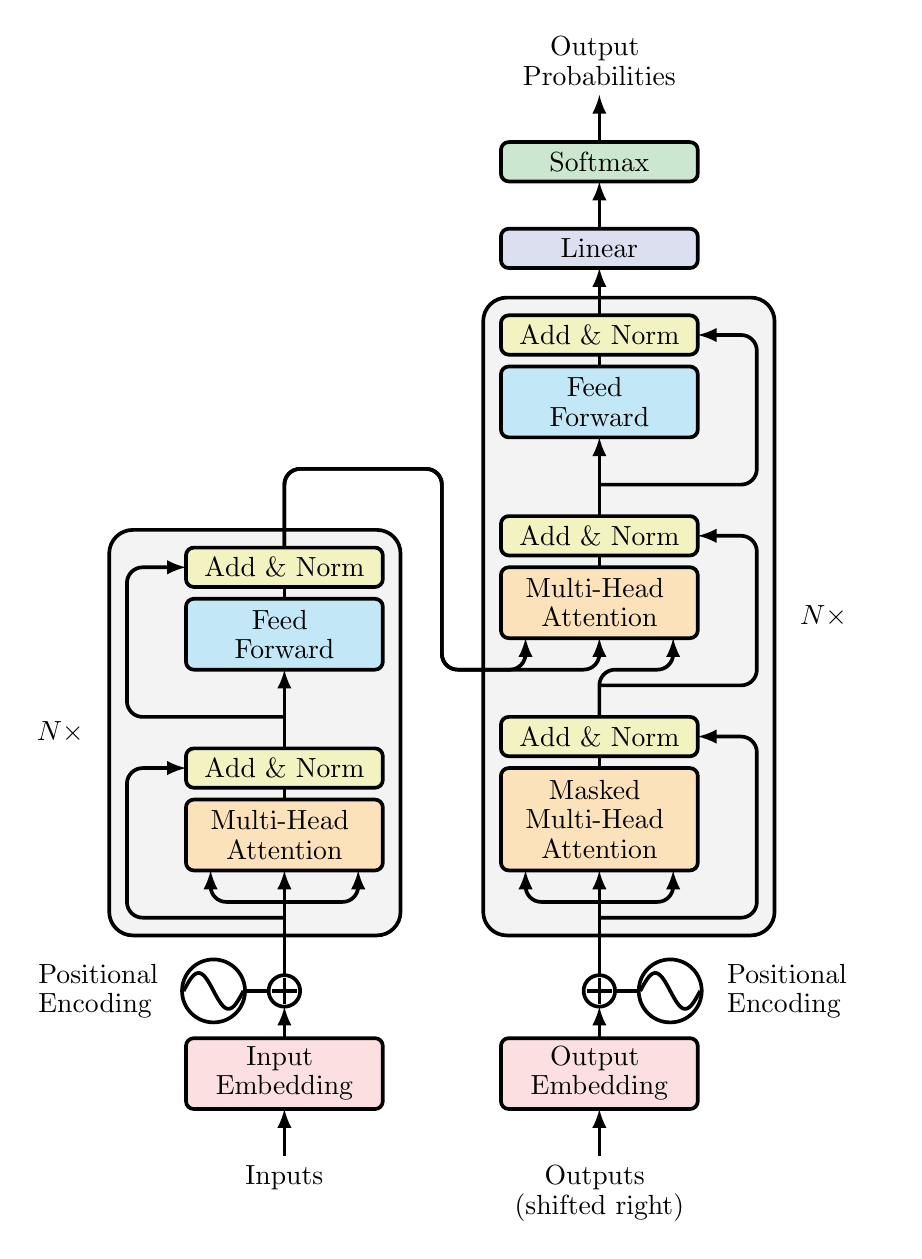
\begin{tikzpicture}
\definecolor{emb_color}{RGB}{252,224,225}
\definecolor{multi_head_attention_color}{RGB}{252,226,187}
\definecolor{add_norm_color}{RGB}{242,243,193}
\definecolor{ff_color}{RGB}{194,232,247}
\definecolor{softmax_color}{RGB}{203,231,207}
\definecolor{linear_color}{RGB}{220,223,240}
\definecolor{gray_bbox_color}{RGB}{243,243,244}
\draw[fill=gray_bbox_color, line width=0.046875cm, rounded corners=0.300000cm] (-0.975000, 6.455000) -- (2.725000, 6.455000) -- (2.725000, 1.305000) -- (-0.975000, 1.305000) -- cycle;
\draw[fill=gray_bbox_color, line width=0.046875cm, rounded corners=0.300000cm] (3.775000, 9.405000) -- (7.475000, 9.405000) -- (7.475000, 1.305000) -- (3.775000, 1.305000) -- cycle;
\draw[line width=0.046875cm, fill=emb_color, rounded corners=0.100000cm] (0.000000, 0.000000) -- (2.500000, 0.000000) -- (2.500000, -0.900000) -- (0.000000, -0.900000) -- cycle;
\node[text width=2.500000cm, align=center] at (1.250000,-0.450000) {Input \vspace{-0.05cm} \linebreak Embedding};
\draw[line width=0.046875cm, fill=emb_color, rounded corners=0.100000cm] (4.000000, 0.000000) -- (6.500000, 0.000000) -- (6.500000, -0.900000) -- (4.000000, -0.900000) -- cycle;
\node[text width=2.500000cm, align=center] at (5.250000,-0.450000) {Output \vspace{-0.05cm} \linebreak Embedding};
\draw[line width=0.046875cm, fill=add_norm_color, rounded corners=0.100000cm] (0.000000, 3.680000) -- (2.500000, 3.680000) -- (2.500000, 3.180000) -- (0.000000, 3.180000) -- cycle;
\node[text width=2.500000cm, align=center] at (1.250000,3.430000) {Add \& Norm};
\draw[line width=0.046875cm, fill=multi_head_attention_color, rounded corners=0.100000cm] (0.000000, 3.030000) -- (2.500000, 3.030000) -- (2.500000, 2.130000) -- (0.000000, 2.130000) -- cycle;
\node[text width=2.500000cm, align=center] at (1.250000,2.580000) {Multi-Head \vspace{-0.05cm} \linebreak Attention};
\draw[line width=0.046875cm] (1.250000, 3.030000) -- (1.250000, 3.180000);
\draw[line width=0.046875cm, fill=add_norm_color, rounded corners=0.100000cm] (4.000000, 6.630000) -- (6.500000, 6.630000) -- (6.500000, 6.130000) -- (4.000000, 6.130000) -- cycle;
\node[text width=2.500000cm, align=center] at (5.250000,6.380000) {Add \& Norm};
\draw[line width=0.046875cm, fill=multi_head_attention_color, rounded corners=0.100000cm] (4.000000, 5.980000) -- (6.500000, 5.980000) -- (6.500000, 5.080000) -- (4.000000, 5.080000) -- cycle;
\node[text width=2.500000cm, align=center] at (5.250000,5.530000) {Multi-Head \vspace{-0.05cm} \linebreak Attention};
\draw[line width=0.046875cm] (5.250000, 5.980000) -- (5.250000, 6.130000);
\draw[line width=0.046875cm, fill=add_norm_color, rounded corners=0.100000cm] (4.000000, 4.080000) -- (6.500000, 4.080000) -- (6.500000, 3.580000) -- (4.000000, 3.580000) -- cycle;
\node[text width=2.500000cm, align=center] at (5.250000,3.830000) {Add \& Norm};
\draw[line width=0.046875cm, fill=multi_head_attention_color, rounded corners=0.100000cm] (4.000000, 3.430000) -- (6.500000, 3.430000) -- (6.500000, 2.130000) -- (4.000000, 2.130000) -- cycle;
\node[text width=2.500000cm, align=center] at (5.250000,2.780000) {Masked \vspace{-0.05cm} \linebreak Multi-Head \vspace{-0.05cm} \linebreak Attention};
\draw[line width=0.046875cm] (5.250000, 3.430000) -- (5.250000, 3.580000);
\draw[line width=0.046875cm, fill=add_norm_color, rounded corners=0.100000cm] (0.000000, 6.230000) -- (2.500000, 6.230000) -- (2.500000, 5.730000) -- (0.000000, 5.730000) -- cycle;
\node[text width=2.500000cm, align=center] at (1.250000,5.980000) {Add \& Norm};
\draw[line width=0.046875cm, fill=ff_color, rounded corners=0.100000cm] (0.000000, 5.580000) -- (2.500000, 5.580000) -- (2.500000, 4.680000) -- (0.000000, 4.680000) -- cycle;
\node[text width=2.500000cm, align=center] at (1.250000,5.130000) {Feed \vspace{-0.05cm} \linebreak Forward};
\draw[line width=0.046875cm] (1.250000, 5.580000) -- (1.250000, 5.730000);
\draw[line width=0.046875cm, fill=add_norm_color, rounded corners=0.100000cm] (4.000000, 9.180000) -- (6.500000, 9.180000) -- (6.500000, 8.680000) -- (4.000000, 8.680000) -- cycle;
\node[text width=2.500000cm, align=center] at (5.250000,8.930000) {Add \& Norm};
\draw[line width=0.046875cm, fill=ff_color, rounded corners=0.100000cm] (4.000000, 8.530000) -- (6.500000, 8.530000) -- (6.500000, 7.630000) -- (4.000000, 7.630000) -- cycle;
\node[text width=2.500000cm, align=center] at (5.250000,8.080000) {Feed \vspace{-0.05cm} \linebreak Forward};
\draw[line width=0.046875cm] (5.250000, 8.530000) -- (5.250000, 8.680000);
\draw[line width=0.046875cm, fill=linear_color, rounded corners=0.100000cm] (4.000000, 10.280000) -- (6.500000, 10.280000) -- (6.500000, 9.780000) -- (4.000000, 9.780000) -- cycle;
\node[text width=2.500000cm, align=center] at (5.250000,10.030000) {Linear};
\draw[line width=0.046875cm, fill=softmax_color, rounded corners=0.100000cm] (4.000000, 11.380000) -- (6.500000, 11.380000) -- (6.500000, 10.880000) -- (4.000000, 10.880000) -- cycle;
\node[text width=2.500000cm, align=center] at (5.250000,11.130000) {Softmax};
\draw[line width=0.046875cm] (1.250000, 0.600000) circle (0.200000);
\draw[line width=0.046875cm] (1.410000, 0.600000) -- (1.090000, 0.600000);
\draw[line width=0.046875cm] (1.250000, 0.760000) -- (1.250000, 0.440000);
\draw[line width=0.046875cm] (5.250000, 0.600000) circle (0.200000);
\draw[line width=0.046875cm] (5.410000, 0.600000) -- (5.090000, 0.600000);
\draw[line width=0.046875cm] (5.250000, 0.760000) -- (5.250000, 0.440000);
\draw[line width=0.046875cm] (0.350000, 0.600000) circle (0.400000);
\draw[line width=0.046875cm] (-0.030000, 0.600000) -- (-0.014490, 0.629156) -- (0.001020, 0.657833) -- (0.016531, 0.685561) -- (0.032041, 0.711884) -- (0.047551, 0.736369) -- (0.063061, 0.758616) -- (0.078571, 0.778258) -- (0.094082, 0.794973) -- (0.109592, 0.808486) -- (0.125102, 0.818576) -- (0.140612, 0.825077) -- (0.156122, 0.827883) -- (0.171633, 0.826946) -- (0.187143, 0.822284) -- (0.202653, 0.813971) -- (0.218163, 0.802145) -- (0.233673, 0.786999) -- (0.249184, 0.768783) -- (0.264694, 0.747796) -- (0.280204, 0.724382) -- (0.295714, 0.698925) -- (0.311224, 0.671845) -- (0.326735, 0.643584) -- (0.342245, 0.614608) -- (0.357755, 0.585392) -- (0.373265, 0.556416) -- (0.388776, 0.528155) -- (0.404286, 0.501075) -- (0.419796, 0.475618) -- (0.435306, 0.452204) -- (0.450816, 0.431217) -- (0.466327, 0.413001) -- (0.481837, 0.397855) -- (0.497347, 0.386029) -- (0.512857, 0.377716) -- (0.528367, 0.373054) -- (0.543878, 0.372117) -- (0.559388, 0.374923) -- (0.574898, 0.381424) -- (0.590408, 0.391514) -- (0.605918, 0.405027) -- (0.621429, 0.421742) -- (0.636939, 0.441384) -- (0.652449, 0.463631) -- (0.667959, 0.488116) -- (0.683469, 0.514439) -- (0.698980, 0.542167) -- (0.714490, 0.570844) -- (0.730000, 0.600000);
\draw[line width=0.046875cm] (6.150000, 0.600000) circle (0.400000);
\draw[line width=0.046875cm] (5.770000, 0.600000) -- (5.785510, 0.629156) -- (5.801020, 0.657833) -- (5.816531, 0.685561) -- (5.832041, 0.711884) -- (5.847551, 0.736369) -- (5.863061, 0.758616) -- (5.878571, 0.778258) -- (5.894082, 0.794973) -- (5.909592, 0.808486) -- (5.925102, 0.818576) -- (5.940612, 0.825077) -- (5.956122, 0.827883) -- (5.971633, 0.826946) -- (5.987143, 0.822284) -- (6.002653, 0.813971) -- (6.018163, 0.802145) -- (6.033673, 0.786999) -- (6.049184, 0.768783) -- (6.064694, 0.747796) -- (6.080204, 0.724382) -- (6.095714, 0.698925) -- (6.111224, 0.671845) -- (6.126735, 0.643584) -- (6.142245, 0.614608) -- (6.157755, 0.585392) -- (6.173265, 0.556416) -- (6.188776, 0.528155) -- (6.204286, 0.501075) -- (6.219796, 0.475618) -- (6.235306, 0.452204) -- (6.250816, 0.431217) -- (6.266327, 0.413001) -- (6.281837, 0.397855) -- (6.297347, 0.386029) -- (6.312857, 0.377716) -- (6.328367, 0.373054) -- (6.343878, 0.372117) -- (6.359388, 0.374923) -- (6.374898, 0.381424) -- (6.390408, 0.391514) -- (6.405918, 0.405027) -- (6.421429, 0.421742) -- (6.436939, 0.441384) -- (6.452449, 0.463631) -- (6.467959, 0.488116) -- (6.483469, 0.514439) -- (6.498980, 0.542167) -- (6.514490, 0.570844) -- (6.530000, 0.600000);
\draw[line width=0.046875cm, -latex] (1.250000, 3.680000) -- (1.250000, 4.680000);
\draw[line width=0.046875cm, -latex] (5.250000, 6.630000) -- (5.250000, 7.630000);
\draw[line width=0.046875cm, -latex] (5.250000, 9.180000) -- (5.250000, 9.780000);
\draw[line width=0.046875cm, -latex] (5.250000, 10.280000) -- (5.250000, 10.880000);
\draw[line width=0.046875cm, -latex] (1.250000, 0.000000) -- (1.250000, 0.400000);
\draw[line width=0.046875cm, -latex] (1.250000, 0.800000) -- (1.250000, 2.130000);
\draw[line width=0.046875cm, -latex] (5.250000, 0.800000) -- (5.250000, 2.130000);
\draw[line width=0.046875cm, -latex] (5.250000, 0.000000) -- (5.250000, 0.400000);
\draw[line width=0.046875cm] (0.750000, 0.600000) -- (1.050000, 0.600000);
\draw[line width=0.046875cm] (5.450000, 0.600000) -- (5.750000, 0.600000);
\draw[-latex, line width=0.046875cm, rounded corners=0.200000cm] (1.250000, 4.080000) -- (-0.750000, 4.080000) -- (-0.750000, 5.980000) -- (0.000000, 5.980000);
\draw[-latex, line width=0.046875cm, rounded corners=0.200000cm] (1.250000, 1.530000) -- (-0.750000, 1.530000) -- (-0.750000, 3.430000) -- (0.000000, 3.430000);
\draw[-latex, line width=0.046875cm, rounded corners=0.200000cm] (5.250000, 1.530000) -- (7.250000, 1.530000) -- (7.250000, 3.830000) -- (6.500000, 3.830000);
\draw[-latex, line width=0.046875cm, rounded corners=0.200000cm] (5.250000, 4.480000) -- (7.250000, 4.480000) -- (7.250000, 6.380000) -- (6.500000, 6.380000);
\draw[-latex, line width=0.046875cm, rounded corners=0.200000cm] (5.250000, 7.030000) -- (7.250000, 7.030000) -- (7.250000, 8.930000) -- (6.500000, 8.930000);
\draw[-latex, line width=0.046875cm, rounded corners=0.200000cm] (1.250000, 1.730000) -- (0.312500, 1.730000) -- (0.312500, 2.130000);
\draw[-latex, line width=0.046875cm, rounded corners=0.200000cm] (1.250000, 1.730000) -- (2.187500, 1.730000) -- (2.187500, 2.130000);
\draw[-latex, line width=0.046875cm, rounded corners=0.200000cm] (5.250000, 1.730000) -- (4.312500, 1.730000) -- (4.312500, 2.130000);
\draw[-latex, line width=0.046875cm, rounded corners=0.200000cm] (5.250000, 1.730000) -- (6.187500, 1.730000) -- (6.187500, 2.130000);
\draw[-latex, line width=0.046875cm, rounded corners=0.200000cm] (1.250000, 6.230000) -- (1.250000, 7.230000) -- (3.250000, 7.230000) -- (3.250000, 4.680000) -- (4.312500, 4.680000) -- (4.312500, 5.080000);
\draw[-latex, line width=0.046875cm, rounded corners=0.200000cm] (1.250000, 6.230000) -- (1.250000, 7.230000) -- (3.250000, 7.230000) -- (3.250000, 4.680000) -- (5.250000, 4.680000) -- (5.250000, 5.080000);
\draw[-latex, line width=0.046875cm, rounded corners=0.200000cm] (5.250000, 4.080000) -- (5.250000, 4.680000) -- (6.187500, 4.680000) -- (6.187500, 5.080000);
\draw[line width=0.046875cm, -latex] (1.250000, -1.500000) -- (1.250000, -0.900000);
\draw[line width=0.046875cm, -latex] (5.250000, -1.500000) -- (5.250000, -0.900000);
\draw[line width=0.046875cm, -latex] (5.250000, 11.380000) -- (5.250000, 11.980000);
\node[text width=2.500000cm, anchor=north, align=center] at (1.250000,-1.500000) {Inputs};
\node[text width=2.500000cm, anchor=north, align=center] at (5.250000,-1.500000) {Outputs \vspace{-0.05cm} \linebreak (shifted right)};
\node[text width=2.500000cm, anchor=south, align=center] at (5.250000,11.980000) {Output \vspace{-0.05cm} \linebreak Probabilities};
\node[anchor=east] at (-1.175000,3.880000) {$N\times$};
\node[anchor=west] at (7.675000,5.355000) {$N\times$};
\node[text width=2.000000cm, anchor=east] at (0.250000,0.600000) {Positional \vspace{-0.05cm} \linebreak Encoding};
\node[text width=2.000000cm, anchor=west] at (6.750000,0.600000) {Positional \vspace{-0.05cm} \linebreak Encoding};
\end{tikzpicture}
}
    \caption[Illustration of the Transformer architecture]{The Transformer
    architecture features an encoder (left) and decoder (right) with stacked
    identical layers. Each layer includes multi-head attention and feed-forward
    sub-layers. Positional encodings are added to input and output embeddings,
    and the final output probabilities are generated via a linear transformation
    and softmax function. Figure adapted from \cite{vaswani2017attention}.} 
    \label{fig:transformer}
\end{figure}

\subsubsection{Input Embedding and Positional Encoding} \label{subsec:input_emb}
Before feeding token sequences to either the encoder or the decoder, they are
preprocessed to the expected input format $\bm{X}$ of self-attention layers.
This is done by the input embedding layer, which turns each token into its
corresponding embedding vector $\bm{x}_i$ of size $d_{model}$. Introduced in
Sec.~\ref{subsec:word_embeddings}, these embedding vectors are learned
continuous numerical representations and form the initial representation of each
input token that will be enhanced as it passes through the Transformer layers.

The input embedding layer really is just an embedding matrix $\bm{E}$ and can be
seen as a simple lookup table. It contains the entire set of embedding vectors
for every token in the vocabulary $V$, resulting in a matrix of shape $|V|
\times d_{model}$. Remember from Sec.~\ref{subsec:word_embeddings} that
tokenized raw text is converted into a sequence of integers, each representing
the position of the token in the vocabulary. An embedding lookup can now be
performed by $\bm{x_i} = \bm{s_i} \bm{E}$ with $\bm{s} _i$ being a
\textit{one-hot encoded} vector of length $|V|$ encoding the integer value of
the current token. A one-hot encoded vector is a binary vector with all the
elements set to 0 except at one position, which is set to 1. This multiplication
effectively selects the row of the embedding matrix $\bm{E}$, which corresponds
to the embedding of the input token. Applied to the entire input sequence, the
embedding layer computes:

\begin{equation} \label{eq:input_embedding}
    \bm{X} = \bm{S} \bm{E}
\end{equation}

with $\bm{S} = [\bm{s}_1^T, \ldots, \bm{s}_n^T]$ being an $n \times |V|$ shaped
matrix whose rows are the one-hot encoded vectors $\bm{s}_i$.

In addition, these embeddings are enriched with a positional encoding that
represents the sequential position of each token. This is necessary because the
Transformer architecture lacks any inherent notion of token order due to the
absence of recurrences and convolutions. Otherwise, the model would not be able
to distinguish between tokens based on their position in the sequence, as the
sequence is processed in parallel. To capture the positional information, we add
a set of real-valued vectors of the same dimensionality $d_{model}$ to the
output of the previous input embedding layer. The authors of
\cite{vaswani2017attention} propose the following sinusoidal functions of
different frequencies for generating the positional encodings:

\begin{align}
    \label{eq:positional_encoding}
    \text{PE}_{(i, 2j)} &= \sin\left(\frac{i}{10000^{2j/d_{model}}}\right) \\
    \text{PE}_{(i, 2j+1)} &= \cos\left(\frac{i}{10000^{2j/d_{model}}}\right)
\end{align}

with $i$ being the position of the token in the sequence and $j$ the dimension
of the positional encoding vector such that $j \in \{1, \ldots, d_{model}\}$.
Consequently, for tokens at even positions, the sine function is used, while for
odd positions the cosine function is applied. The use of these sinusoidal
functions is driven by their linear characteristics, which facilitate the
model's ability to learn positional relationships between tokens. However,
alternative methods can also be employed to compute positional encodings.

\subsubsection{Encoder}
The encoder is responsible for mapping the input sequence $\bm{X} = [\bm{x}_1^T,
\ldots, \bm{x}_n^T]$ into an abstract high-dimensional representation $\bm{H} =
[\bm{h}_1^T, \ldots, \bm{h}_n^T]$ of the same dimensionality. It consists of a
stack of $N$ identical layers to make deeper and more powerful networks,
producing more expressive representations. Each layer in the encoder contains
two sub-layers: a non-masked Multi-Head Attention layer followed by a
feed-forward network. Around each sub-layer there is a residual connection
followed by a layer normalization, which helps to stabilize the training
process. The residual connection is a direct connection from the input to the
output of a sub-layer. In order to facilitate the flow of information through
the residual connections and stacks of layers, input and output dimensions of
each sub-layer are identical. Using mathematical notation, a single encoder
layer is expressed as:

\begin{align}
    \label{eq:encoder1}
    \bm{T}_E^{MH} &= \text{MultiHeadAttention}(\bm{X}) \\    
    \bm{T}_E^{LN} &= \text{LayerNorm}(\bm{X} + \bm{T}_E^{MH}) \\
    \bm{T}_E^{FF} &= \text{FeedForward}(\bm{T}_E^{LN}) \\
    \label{eq:encoder2}
    \text{Encoder}(\bm{X}) &= \text{LayerNorm}(\bm{T}_E^{LN} + \bm{T}_E^{FF})
\end{align}

where $\bm{T}_E^{MH}$, $\bm{T}_E^{LN}$ and $\bm{T}_E^{FF}$ denote the
intermediate outputs of the \textit{MultiHeadAttention}, \textit{LayerNorm} and
\textit{FeedForward} sub-layers, respectively. Multi-Head Attention is computed
as defined in Eq.~\ref{eq:decoder_mh}-\ref{eq:mh_attention2}. The feed-forward
network is a simple fully connected neural network with two layers and an $ReLU$
activation function:

\begin{equation}
    \text{FeedForward}(\bm{X}) = \text{ReLU}(\bm{X} \bm{W}_1 + \bm{b}_1) \bm{W}_2 + \bm{b}_2
\end{equation}

with $\bm{W}_1 \in \mathbb{R}^{d_{model} \times d_{ff}}$, $\bm{b}_1 \in
\mathbb{R}^{d_{ff}}$, $\bm{W}_2 \in \mathbb{R}^{d_{ff} \times d_{model}}$ and
$\bm{b}_2 \in \mathbb{R}^{d_{model}}$ being the respective weight and bias for
each of the two layers. The size of the hidden layer $d_{ff}$ is typically
chosen to be larger than the model dimensionality $d_{model}$, e.g. in the
original Transformer $d_{ff} = 2048$.

Layer normalization is applied simultaneously to each row of a sub-layer's
output with respect to the mean $\mu$ and standard deviation $\sigma$ of the
row:

\begin{equation}
    \text{LayerNorm}(\bm{x}_i) = \gamma \cdot \frac{\bm{x}_i - \mu}{\sigma} + \beta, 
    \quad \forall i \ 1 \leq i \leq n
\end{equation}

where $\gamma$ and $\beta$ are two learnable parameters representing gain and
offset.

To obtain the final encoder output $\bm{H}$ the encoder layer defined in
Eq.~\ref{eq:encoder1}-\ref{eq:encoder2} is successively applied $N$ times:

\begin{equation}
    % \bm{H} = \underbrace{\text{Encoder}(\ldots \text{Encoder}(\text{Encoder}}_{N}(\bm{X})))
    \bm{H} = \left(\underbrace{\text{Encoder} \circ \ldots \text{Encoder} \circ \text{Encoder}}_{N}\right)(\bm{X})
\end{equation}

\subsubsection{Decoder}
In contrast to the encoder, the decoder processes its input sequence
autoregressively and not in parallel. This means that the decoder generates a
sequence of outputs, one token at a time, while at time step $i$ the preceding
output token from time step $i-1$ is taken as an additional input. The decoder
also consists of $N$ identical layers, each containing three sub-layers: a
masked Multi-Head Attention layer, a Multi-Head Attention layer, and a
feed-forward network. Encoder and decoder layers are similar in structure, but
the decoder has an additional masked Multi-Head Attention sub-layer that attends
to the output of the previous decoder layer. This is necessary to prevent the
model from attending to future tokens during prediction for the next token.
Furthermore, decoder and encoder are connected by passing the encoder output
$\bm{H}$ to the Multi-Head Attention layer and serves as the key and value
parameters (refer to Eq.~\ref{eq:decoder_mh}). More formally, the decoder layer
is defined as:

\begin{align}
    \label{eq:decoder1}
    \bm{t}_i^{MMH} &= \text{MaskedMultiHeadAttention}(\bm{o}_{i-1}) \\ 
    \bm{t}_i^{LN1} &= \text{LayerNorm}(\bm{o}_{i-1} + \bm{t}_i^{MMH}) \\
    \label{eq:decoder_mh}
    \bm{t}_i^{MH} &= \text{MultiHeadAttention}(\bm{h}_i, \bm{h}_i, \bm{t}_i^{LN1}) \\
    \bm{t}_i^{LN2} &= \text{LayerNorm}(\bm{t}_i^{LN1} + \bm{t}_i^{MH}) \\
    \bm{t}_i^{FF} &= \text{FeedForward}(\bm{t}_i^{LN2}) \\
    \label{eq:decoder2}
    \text{Decoder}(\bm{h}_i, \bm{o}_{i-1}) &= \text{LayerNorm}(\bm{t}_i^{LN2} + \bm{t}_i^{FF})
\end{align}

with $\bm{o}_{i-1}$ being the previous decoder output at time step $i-1$ and
$\bm{h}_i$ the encoder output at time step $i$ and $1 \leq i \leq n$. Again,
intermediate outputs are denoted by $\bm{t}_i^{MMH}$, $\bm{t}_i^{LN1}$,
$\bm{t}_i^{MH}$, $\bm{t}_i^{LN2}$ and $\bm{t}_i^{FF}$. Multi-Head Attention,
layer normalization and feed-forward layers are defined as in the encoder.

The decoder output $\bm{o}_i$ is obtained by $N$ consecutive applications of the
decoder layer:

\begin{equation}
    \bm{o}_i = \left(\underbrace{\text{Decoder} \circ \ldots \text{Decoder} \circ \text{Decoder}}_{N}\right)(\bm{h}_i, \bm{o}_{i-1})
\end{equation}

\subsubsection{Language Modeling Head}
For the purpose of model training, the last component in the Transformer
architecture is the language modeling head. Thinking back to Sec.~\ref{sec:lm},
the goal of language modeling is to predict the next token in a sequence given
the preceding tokens. More precisely, language models compute a conditional
probability for every possible next token, giving us a probability distribution
over the entire vocabulary. The language modeling head computes the distribution
by taking the final output at the last decoder layer $\bm{o}_n$, which contains
the context as abstract representation of the input sequence, and applying a
linear transformation followed by a softmax function:

\begin{align}
    \bm{u} &= \bm{o}_n \bm{E}^T \label{eq:unembedding} \\
    \bm{\hat{y}} &= \text{softmax}(\bm{u}) \label{eq:lm_softmax}
\end{align}

The linear transformation in Eq.~\ref{eq:unembedding} acts as a classifier which
assigns a score to each token in the vocabulary $V$ collected in the
\textit{logits} vector $\bm{u}$ of length $|V|$. Observe how we use the
transpose of the embedding matrix $\bm{E}$ of shape $d_{model} \times |V|$ as
the mapping weights. Here, the technique of \textit{weight tying} is utilized to
tie the weights of the linear transformation in the language modeling head to
the embedding matrix from Eq.~\ref{eq:input_embedding}. During model training,
$\bm{E}$ will be optimized on both the input and output side, which is why
$\bm{E}^T$ is referred to as the \textbf{unembedding} layer. In
Eq.~\ref{eq:lm_softmax}, a softmax function normalizes the logits $\bm{u}$ into
output probabilities over the vocabulary, resembling the predicted token
distribution $\hat{\bm{y}}$. 

These probabilities $\hat{\bm{y}}$ can then be used in the learning process by
calculating the \textbf{cross-entropy loss} between the predicted and actual
token distribution $\bm{y}$. We obtain the true next token from the natural
sequence of words in the training data, which is why we say the model is trained
in a \textbf{self-supervised} manner. The cross-entropy loss of a token sequence
of length $n$ is defined as:

\begin{align}
    \mathcal{L} &= \frac{1}{n}\sum_{i = 1}^{n}L_i^{CE} \\
    L_i^{CE}(\hat{\bm{y}}_i, \bm{y}_i) &= -\sum_{w \in V} \bm{y}_i[w] \log\hat{\bm{y}}_i[w] \\
    &= -\log\hat{\bm{y}}_i[w_{i+1}]
\end{align}

where $\bm{y}_i$ is the one-hot encoded vector of the true next token at
sequence position $i$, which simplifies the loss $L_i^{CE}$ to the negative log
probability that the Transformer assigns to the next word token $w_{i+1}$.
Subsequently, the loss is minimized by adjusting all learnable model parameters,
i.e. the weights of the Transformer layers, through
backpropagation~\cite{rumelhart1986learning}.

\subsubsection{Model Variations}
A major benefit of Transformers is that the encoder and decoder can be separated
and used as independent models \cite{min2023recent}. This has led to the
development of several Transformer-based language models featuring all or only
selected Transformer components as shown in Fig~\ref{fig:llm_types}. In the
following, we will briefly describe the different types:

\begin{figure}[htb]
    \centering
    \begin{subfigure}{0.24\textwidth}
        \centering
        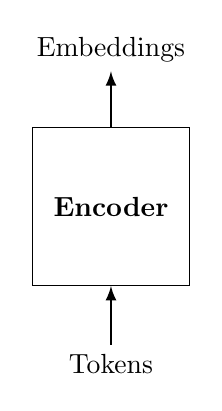
\begin{tikzpicture}[
    block/.style={draw, rectangle, minimum width=2cm, minimum height=2cm, text centered, font=\bfseries},
    arrow/.style={->, >=latex, thick}
]

% Encoder block
\node[block] (encoder) at (0, 0) {Encoder};

% Tokens input
\node at (0, -2) (tokens) {Tokens};
\draw[arrow] (tokens) -- (encoder.south);

% Embeddings output
\node at (0, 2) (embeddings) {Embeddings};
\draw[arrow] (encoder.north) -- (embeddings);

\end{tikzpicture}
 
        \caption{Encoder}
    \end{subfigure}
    \hfill
    \begin{subfigure}{0.24\textwidth}
        \centering
        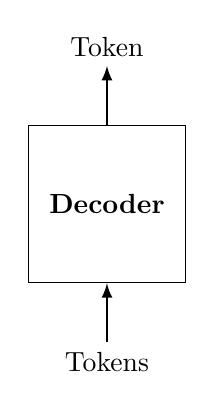
\begin{tikzpicture}[
    block/.style={draw, rectangle, minimum width=2cm, minimum height=2cm, text centered, font=\bfseries},
    arrow/.style={->, >=latex, thick}
]

% Decoder block
\node[block] (encoder) at (0, 0) {Decoder};

% Tokens input
\node at (0, -2) (tokens) {Tokens};
\draw[arrow] (tokens) -- (encoder.south);

% Embeddings output
\node at (0, 2) (token) {Token};
\draw[arrow] (encoder.north) -- (token);

\end{tikzpicture}
 
        \caption{Decoder}
    \end{subfigure}
    \hfill
    \begin{subfigure}{0.49\textwidth}
        \centering
        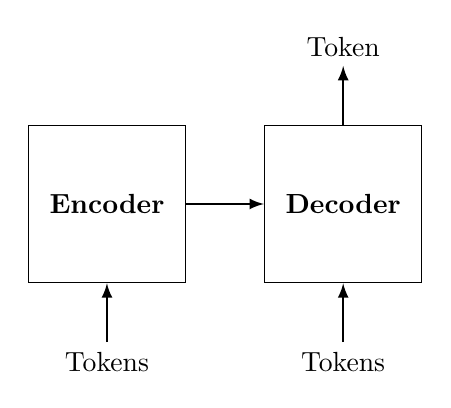
\begin{tikzpicture}[
    block/.style={draw, rectangle, minimum width=2cm, minimum height=2cm, text centered, font=\bfseries},
    arrow/.style={->, >=latex, thick}
]

% Encoder block
\node[block] (encoder) at (0, 0) {Encoder};

% Decoder block
\node[block] (decoder) at (3, 0) {Decoder};

% Tokens input for Encoder
\node at (0, -2) (encoder_input) {Tokens};
\draw[arrow] (encoder_input) -- (encoder.south);

% Tokens input for Decoder
\node at (3, -2) (decoder_input) {Tokens};
\draw[arrow] (decoder_input) -- (decoder.south);

% Token output from Decoder
\node at (3, 2) (decoder_output) {Token};
\draw[arrow] (decoder.north) -- (decoder_output);

% Connection between Encoder and Decoder
\draw[arrow] (encoder.east) -- (decoder.west);

\end{tikzpicture}
 
        \caption{Encoder-Decoder}
    \end{subfigure}
    \caption{Architectural variations of the Transformer}
    \label{fig:llm_types}
\end{figure}

\paragraph{Encoder-Decoder}
Encoder-decoder models follow the original Transformer architecture introduced
in Sec.~\ref{sec:architecture} consisting of two primary components: an encoder
that reads and processes the input sequence and a decoder responsible for
generating the output sequence. The encoder part aims to capture the important
information and context of the input sequence and then generates the context
vector. The decoder decodes this vector and generates the output sequence one
token at a time while maintaining the prior generated tokens along with the
context vector. A notable example language model is T5
\cite{raffel2020exploring}, which utilizes this model type in
sequence-to-sequence tasks such as translation or question answering. Apart from
text, the Transformer is also applied to tasks in other modalities such as
speech \cite{toshniwal2018comparison} and image recognition
\cite{dosovitskiy2021image}.

\paragraph{Encoder-only}
Encoder-only models are based solely on the encoder part of the Transformer
architecture. The encoder processes and encodes the input sentence into a hidden
representation that grasps the connections between words and the overall context
of the sentence. For instance, BERT \cite{devlin2019bert} and its extensions,
RoBERTa \cite{liu2019roberta} and DistilBERT \cite{sanh2019distilbert}, are well
suited for tasks that involve understanding the input text rather than
generating new text. Examples of successful applications include sentiment
analysis \cite{yuan2023revisiting,clark2020electra} and named entity recognition
\cite{wu2020scalable, zhang2022knowledge}.

\paragraph{Decoder-only}
Decoder-only models utilize the decoder component of the Transformer. Unlike
encoder-only models that are good at summarizing, i.e. learning patterns in the
input data and analyzing the text, decoder-only models generate text by
predicting the next tokens in a sequence based on previous tokens
\cite{radford2018improving}. To generate a token, the decoder's output
probabilities are sampled from, e.g. the token with the highest probability
(greedy decoding). From this, a sequence of text can be generated token by token
by passing the output tokens as inputs back into the decoder. The GPT models
\cite{radford2019gpt2, brown2020language, achiam2023gpt} are the first examples
of decoder-only models that have been used for text generation. Other instances
of decoder-only LMs include the open-source LLaMA family
\cite{touvron2023llama1, touvron2023llama2, dubey2024llama3} developed by Meta.
